\title{Project 1 Report: Scanner/Parser}
\author{Jack Choi, Allen Mi, Hanxiang Ren}
\date{September 25, 2018}
\newcommand{\reportfile}{scalars_report_1.tex}
\documentclass[letterpaper, 11pt]{article}
\usepackage{geometry}
\geometry{letterpaper, portrait, margin=1.2in}

\makeatletter

\usepackage{fullpage}
\usepackage{multirow}
\usepackage{adjustbox}
\usepackage{tabularx}

\usepackage{amsmath}
\usepackage{amssymb}
\usepackage{amsthm}

\usepackage{graphicx}
\usepackage{listings}
\usepackage{xcolor}
\usepackage{titlesec}

\setcounter{secnumdepth}{4}

\titleformat{\paragraph}
{\normalfont\normalsize\bfseries}{\theparagraph}{1em}{}
\titlespacing*{\paragraph}
{0pt}{3.25ex plus 1ex minus .2ex}{1.5ex plus .2ex}

\lstset{
    frameround=fttt,
    language=scala,
    numbers=left,
    breaklines=true,
    keywordstyle=\color{black}\bfseries, 
    basicstyle=\ttfamily\color{black},
    numberstyle=\color{black}
}
\lstMakeShortInline|

\newcommand{\docinitiated}{\@date}
\newcommand{\doctitle}{\@title}
\newcommand{\docauthors}{\@author}

\begin{document}
    \noindent
    \begin{tabularx}{\textwidth}{X r}
        \hspace{-0.1in}
        \begin{adjustbox}{valign=t}
            
\includegraphics[width=0.23\textwidth]{img/scalars_logo.png}
        \end{adjustbox}
        \multirow{3}{0.75\textwidth}{
            \raggedleft\large\textbf{\doctitle} \\
            \normalsize\docauthors \\
            \docinitiated
        }
    \end{tabularx}
    \hspace{0.2in}
    \makeatother
    % \input{\reportfile}

\tableofcontents

\section{Dataflow Optimizations}

The Scalars Decaf Compiler implements 4 classes of dataflow optimizations, arranged in scope from micro- to macro-level. The classes are as detailed below:

\subsection{Peephole Optimizations}

Peephole optimizations are the smallest in scope: They consider a close vicinity of the target code in the control-flow diagram (CFG). The peephole optimizations implemented are listed as follows.

\subsubsection{Virtual CFG Node Elimination}

\paragraph{Introduction}

Virtual CFG nodes, especially |nop| nodes, are generated when translating the intermediate representation (IR) structure to the CFG. The virtual CFG node elimination discards these virtual nodes and prepare the CFG for assembly code translation. The process of performing this optimization is detailed in page 57 of L12.

\paragraph{Implementation Details}

The implementation can be found in |src/codegen/PeepHole.scala|. The optimization is performed via traversing the entire CFG structure. Once a suitable virtual CFG node (target) is discovered, the parents and children of the target are linked together and the target is removed.

\paragraph{Demonstration}
\begin{figure}[ht]
    \centering
    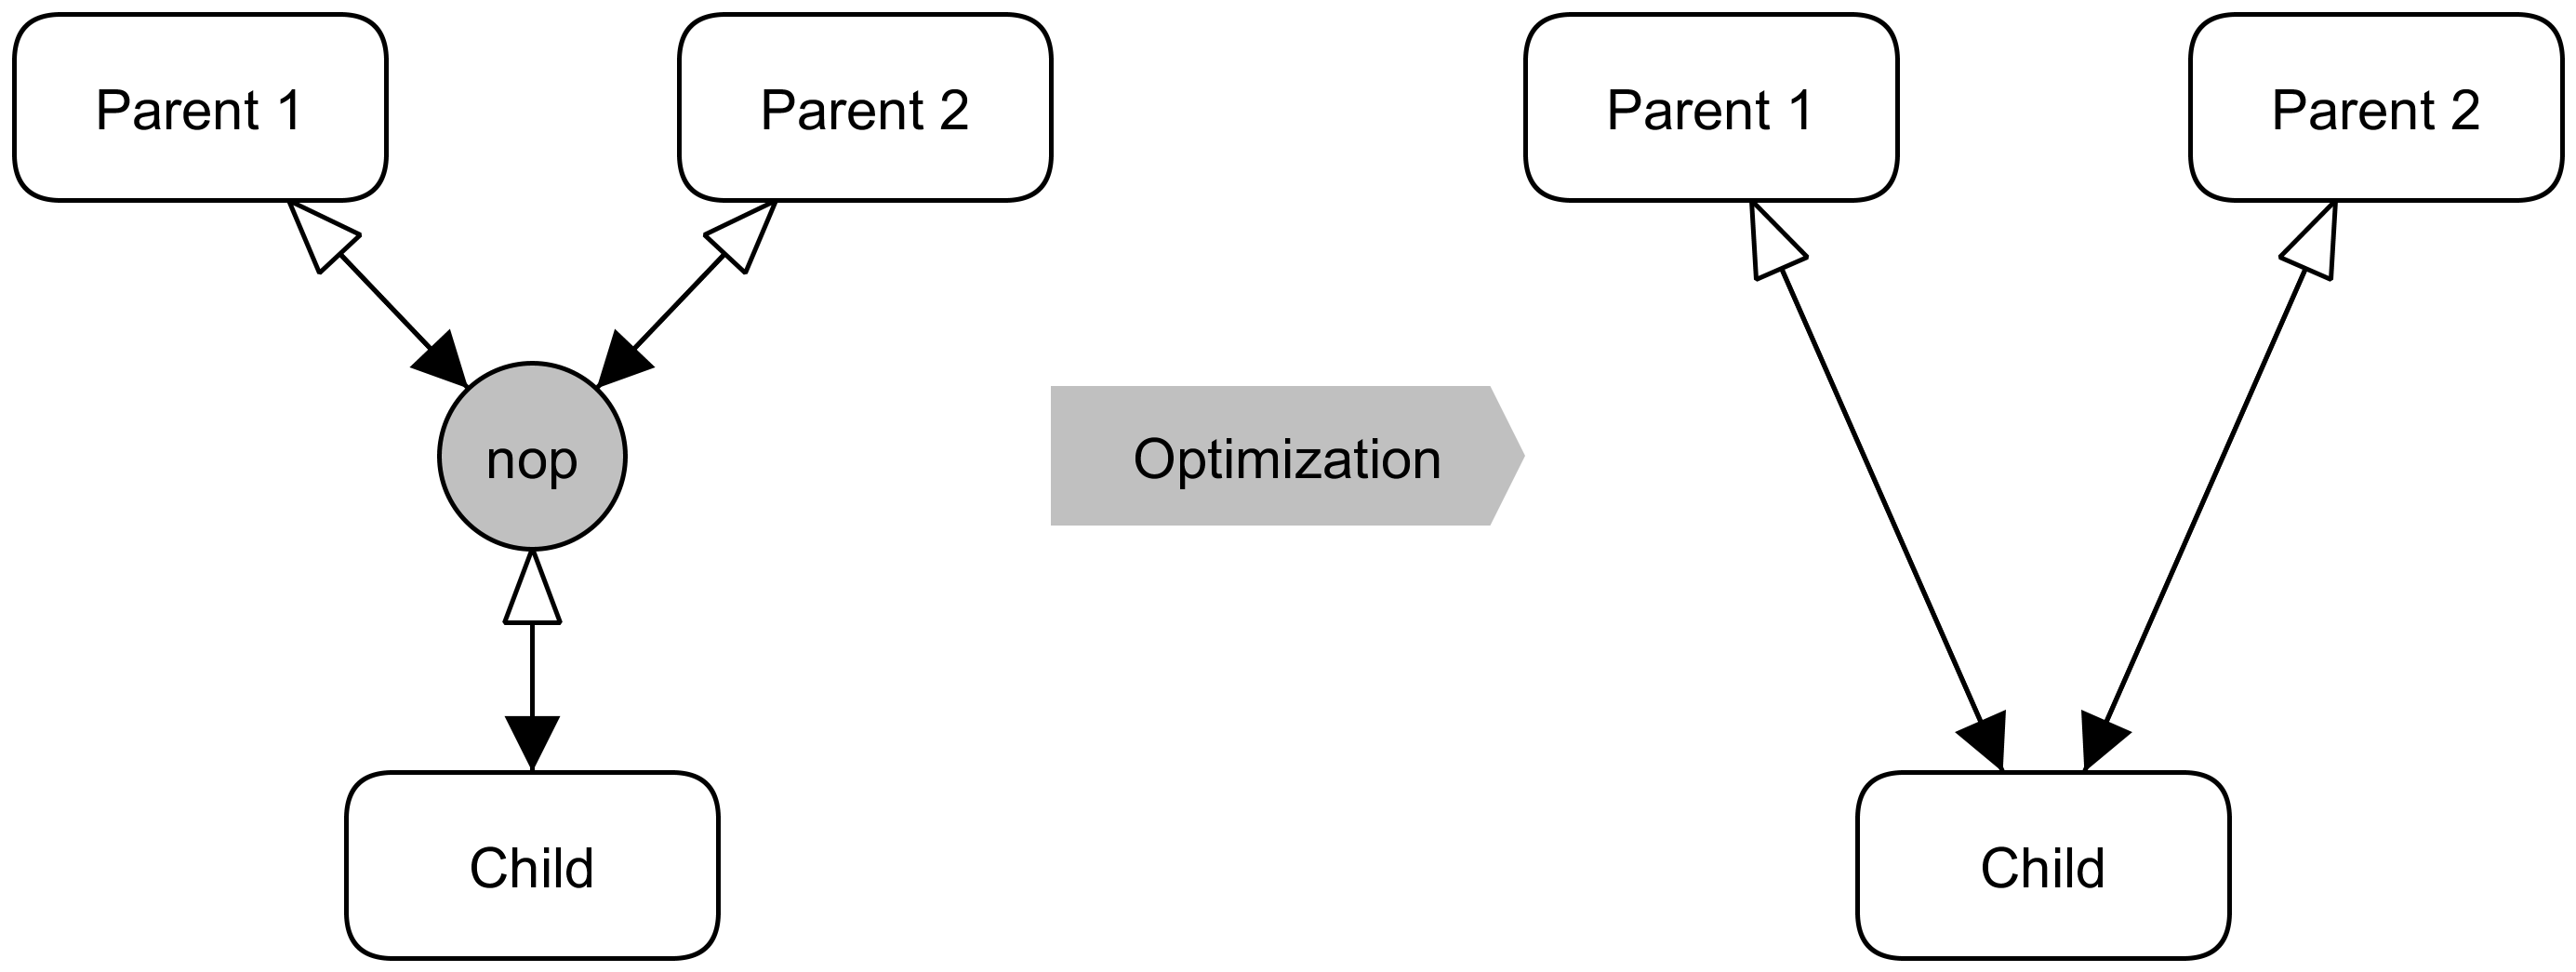
\includegraphics[width=0.75\textwidth]{img/virtual-cfg-node-elimination}
    \caption{A demonstration of virtual CFG node elimination}
    \label{fig:virtual-cfg-node-elimination}
\end{figure}
Figure \ref{fig:virtual-cfg-node-elimination} demonstrates the process of eliminating a |nop| node and linking its parents and child.


\subsubsection{Constant Folding}

\paragraph{Introduction}

This optimization scans for assignments of constant-operand expressions to variables and evaluate the expressions at compile-time rather than run-time. Since constant folding only occurs when the operands are integer of Boolean literals, substituting run-time evaluation with compile-time evaluation does not impact the value of the expression. Performance gain is achieved by reducing the amount of work needed at run-time.

\paragraph{Implementation Details}

The implementation can be found in |src/optimization/ConstantFolding.scala|. The implementation is performed by traversing the CFG structure. Upon encountering an operation, the program checks whether the operand(s) is/are integer or Boolean literals. If this is the case, the expression is evaluated on-site, and is substituted by an integer or Boolean literal derived from the result of the evaluation.

\paragraph{Demonstration}
The following code listing demonstrates constant folding:

\begin{itemize}
    \item Before optimization:
    \begin{lstlisting}[language=C]
        ...
        bool a;
        int b;
        a = true || false;
        b = 1 + 2;
        ...
    \end{lstlisting}
    \item After optimization:
    \begin{lstlisting}[language=C]
        ...
        bool a;
        int b;
        a = true;
        b = 3;
        ...
    \end{lstlisting}
\end{itemize}

\subsection{Local Optimizations}

The class of local optimizations operate within each block of the CFG. The data structures established when performing local optimizations have a single-block lifespan, and the effect of local optimizations are contained within a single CFG block. The local optimizations are listed as follows:

\subsubsection{Local Common Subexpression Elimination}

\paragraph{Introduction}

When a subexpression is encountered more than once within a single CFG block, the local common subexpression elimination (local CSE) checks whether any of the operands of the said subexpression is reassigned after the subexpression's first evaluation. If not, then it is safe to reuse the results from the previous evaluation. In this case, the local CSE replaces this occurrence of the subexpression with a temporary variable, whose value is assigned when the subexpression is first evaluated.

\paragraph{Implementation Details}

The implementation can be found in |src/optimization/CSE.scala|. The details regarding implementing local CSE can be found in pages 26-33 of L15. The optimization is performed by traversing the CFG structure and identifying each CFG block. Upon entering each block, the program scans all statements sequentially, while maintaining the |var2Val|, |exp2Val|, |exp2Tmp| maps. The substitution is performed by checking |exp2tmp| and substituting the target expression with the corresponding temporary variable.

\paragraph{Demonstration}

The following code listing demonstrates local CSE:

\begin{itemize}
    \item Before optimization:
    \begin{lstlisting}[language=C]
        ...
        int a, b, c, d;
        ...
        c = a * b;
        d = a * b;
        ...
    \end{lstlisting}
    \item After optimization:
    \begin{lstlisting}[language=C]
        ...
        int a, b, c, d;
        ...
        c = a * b;
        t1 = c;
        d = t1;
        ...
    \end{lstlisting}
\end{itemize}

\subsubsection{Local Copy Propagation}

\paragraph{Introduction}

Local copy propagation (local CP) is used to simplify the code structure after local CSE is performed. In local CSE, when a temporary variable is assigned to a subexpression, later use of the subexpression will be replaced by the temporary variable, given that none of the operands are reassigned. However, if the subexpression is already assigned to a program variable when it's first evaluated, and the program variable is not reassigned afterwards until the reuse, we may simply substitute the reuse with program variable rather than the temporary variable.

\paragraph{Implementation Details}

The implementation can be found in |src/optimization/CP.scala|. The details regarding implementing local CP can be found in pages 36-43 of L15. The optimization is performed by traversing the CFG structure and identifying each CFG block. Upon entering each block, the program scans all statements sequentially, while maintaining the |tmp2Var| and |var2Set| maps. The substitution is performed by checking |tmp2Var| and substituting the temporary variable usage with the corresponding program variable.

\paragraph{Demonstration}

The following code listing demonstrates local CP:

\begin{itemize}
    \item Before optimization:
    \begin{lstlisting}[language=C]
        ...
        int a, b, c, d;
        ...
        c = a * b;
        t1 = c;
        d = t1;
        ...
    \end{lstlisting}
    \item After optimization:
    \begin{lstlisting}[language=C]
        ...
        int a, b, c, d;
        ...
        c = a * b;
        t1 = c;
        d = c;
        ...
    \end{lstlisting}
\end{itemize}

\subsubsection{Local Dead Code Elimination}

\paragraph{Introduction}

Within a CFG block, some temporary variables generated by local CSE may not be referenced anywhere. Additionally, some temporary variable usage may be eliminated by performing local CP. Since all temporary variables are not referenced outside its CFG block, we may safely remove the creation of those temporary variables that are not referenced within its CFG block via local dead code elimination (local DCE).

\paragraph{Implementation Details}

The implementation can be found in |src/optimization/DCE.scala|. The details regarding implementing local DCE can be found in pages 45-55 of L15. The optimization is performed by traversing the CFG structure and identifying each CFG block. Upon entering each block, the program scans all statements in reverse order, while maintaining a needed set. After going through all statements, the program eliminates the temporary variable assignments that are never used.

\paragraph{Demonstration}

The following code listing demonstrates local DCE:

\begin{itemize}
    \item Before optimization:
    \begin{lstlisting}[language=C]
        ...
        int a, b, c, d;
        ...
        c = a * b;
        t1 = c;
        d = c;
        ...
    \end{lstlisting}
    \item After optimization:
    \begin{lstlisting}[language=C]
        ...
        int a, b, c, d;
        ...
        c = a * b;
        d = c;
        ...
    \end{lstlisting}
\end{itemize}

\subsection{Global Optimizations}

The class of global optimizations operate within the scope of the program and each method. Program-wide dataflow analysis is required to perform global optimizations. All optimizations of the class depend on a common worklist algorithm that generates |GEN| and |KILL| (|DEF| and |USE| for global dead code elimination) sets given |IN| and |OUT| sets. The global optimizations are listed as follows:

\subsubsection{Global Common Subexpression Elimination}

\paragraph{Introduction}

The global common subexpression elimination (global GCE) is used to simplify the code structure when the same subexpression is evaluated more than once, and the first evaluation is determined available from the perspective of the second evaluation. In this case, the program substitutes the second evaluation with the results from the first evaluation.

\paragraph{Implementation Details}

The implementation can be found in |src/optimization/GlobalCSE.scala|. The details regarding implementing global CSE can be found in pages 24-50 of L17. The optimization is performed by traversing the CFG structure and maintaining the |GEN| and |KILL| sets for each block. After traversing all blocks, the program establishes a worklist with set intersection as its confluence operator. |IN| and |OUT| sets for each block is then generated, and substitutions are carried out based on the |IN| and |OUT| sets for each block.

\paragraph{Demonstration}

The following code listing demonstrates global CSE:

\begin{itemize}
    \item Before optimization:
    \begin{lstlisting}[language=C]
        ...
        int a, b, c, d, e, f, g, h;
        bool k;
        ...
        e = a * b;
        f = c * d;
        if (k) {
            c += 1;
        }
        g = a * b;
        h = c * d;
        ...
    \end{lstlisting}
    \item After optimization:
    \begin{lstlisting}[language=C]
        ...
        int a, b, c, d, e, f, g, h;
        bool k;
        ...
        e = a * b;
        f = c * d;
        if (k) {
            c += 1;
        }
        g = e;
        h = c * d;
        ...
    \end{lstlisting}
\end{itemize}

\subsubsection{Global Copy Propagation}

\paragraph{Introduction}

The global copy propagation (global CP) simplifies program structure by replacing variable references with constants or variable definitions a level shallower. This helps simplify the program structure, increase run-time efficiency, and free-up unused definitions for removal by global dead code elimination.

\paragraph{Implementation Details}

The implementation can be found in |src/optimization/GlobalCP.scala|. The details regarding implementing global CP can be found in pages 8-22 of L17. The optimization is performed by traversing the CFG structure and maintaining the |GEN| and |KILL| sets for each block. After traversing all blocks, the program establishes a worklist with set union as its confluence operator. |IN| and |OUT| sets for each block is then generated, and substitutions are carried out based on the |IN| and |OUT| sets for each block.

\paragraph{Demonstration}

The following code listing demonstrates global CP:

\begin{itemize}
    \item Before optimization:
    \begin{lstlisting}[language=C]
        ...
        int a, b, c, d;
        bool k;
        ...
        a = 1;
        b = 2;
        if (k) {
            b += 1;
        }
        c = a;
        d = b;
        ...
    \end{lstlisting}
    \item After optimization:
    \begin{lstlisting}[language=C]
        ...
        int a, b, c, d;
        bool k;
        ...
        a = 1;
        b = 2;
        if (k) {
            b += 1;
        }
        c = 1;
        d = b;
        ...
    \end{lstlisting}
\end{itemize}

\subsubsection{Global Dead Code Elimination}

\paragraph{Introduction}

The global dead code elimination (global DCE) is used to eliminate the assignments of variables that are not used anywhere later within the program. This help increase run-time efficiency of the code.

\paragraph{Implementation Details}

The implementation can be found in |src/optimization/GlobalDCE.scala|. The details regarding implementing global DCE can be found in pages 53-65 of L17. The optimization is performed by traversing the CFG structure and maintaining the |DEF| and |USE| sets for each block. After traversing all blocks, the program establishes a reverse-order worklist with set union as its confluence operator. |IN| and |OUT| sets for each block is then generated, and eliminations are carried out based on the |IN| and |OUT| sets for each block.

\paragraph{Demonstration}

The following code listing demonstrates global DCE:

\begin{itemize}
    \item Before optimization:
    \begin{lstlisting}[language=C]
        import printf;
        ...
        int a, b, c;
        bool k;
        ...
        a = 1;
        b = 2;
        c = a + b;
        if (k) {
            b += a;
        }
        ...
        printf("%d", b);
        ...
    \end{lstlisting}
    \item After optimization:
    \begin{lstlisting}[language=C]
        import printf;
        ...
        int a, b, c;
        bool k;
        ...
        a = 1;
        b = 2;
        if (k) {
            b += a;
        }
        ...
        printf("%d", b);
        ...
    \end{lstlisting}
\end{itemize}

\subsubsection{Loop Invariant Code Hoisting}

\paragraph{Introduction}

For each loop, the loop invariant code hoisting (LICH) identifies the set of code in the loop body that does not change between iterations. It then moves the set of code to a pre-header of the loop, prompting them to execute once in total, rather than once per iteration.

\paragraph{Implementation Details}

LICH is implemented in |src/optimization/loop_opt/*|, via |InvariantOpt.scala| and |LoopConstruction.scala|. Upon entering a method, the program first construct a representation of each loop within the method. The details for constructing the dominant tree can be found in pages 3-16 of L20. The loop representations are constructed in accordance with pages 17-20 of L20. Afterwards, the program constructs a preheader for each loop and scans for invariant code in the loop body. Any invariant code is then copied to the preheader and marked for removal. When this process is completed, the program eliminates all code marked for removal and returns.

\paragraph{Demonstration}

The following code listing demonstrates LICH:

\begin{itemize}
    \item Before optimization:
    \begin{lstlisting}[language=C]
        ...
        int i;
        bool k;
        k = true;
        ...
        i = 0;
        while (i <= 5) {
            k = false;
            i++;
        }
        ...
    \end{lstlisting}
    \item After optimization:
    \begin{lstlisting}[language=C]
        ...
        int i;
        bool k;
        k = true;
        ...
        i = 0;
        k = false;
        while (i <= 5) {
            i++;
        }
        ...
    \end{lstlisting}
\end{itemize}

\subsection{Meta-Optimizations}
The class of meta-optimizations serve to organize and schedule all other optimizations. They serve as an ``optimization for optimizations'' in some sense. Optimization scheduling is currently the only member of this class.

\subsubsection{Optimization Scheduling}

\paragraph{Introduction}

Optimization scheduling provides a solution to the problem of incomplete optimization. When an optimization is performed once on a set of code, it is not guaranteed that it finds all to-be-optimized instances. This effect could mainly be attributed to nested code structure. However, it is difficult to implement an a priori method for generic implementations to determine the number of necessary iterations. Optimization scheduling solves this problem by determining the sequence of optimizations on-the-fly. It only requires each optimization to report whether it has performed changes within the current iteration.

\paragraph{Implementation Details}

The implementation of optimization scheduling can be found in |src/optimization/RepeatOptimization.scala|, as well as |src/compile/Compiler.scala| and |src/compile/GenerateOptVec.scala|. It also leverages the reset optimization utility in |src/compile/optimization/ResetOptimization.scala|. optimization scheduling groups each \textit{phase} of optimizations into a tuple of 3 vectors. The \textit{prelude} vector contains optimizations that will run at the beginning of each iteration, regardless of its members' reports. Similarly, the \textit{postlude} vector contains optimizations that will run at the end of each iteration, regardless of its members' reports. The \textit{condition} vector contains optimizations that determine how this optimization tuple would run. After each iteration, the program queries each optimization regarding whether a change has occurred. If any optimization reports positively, a new iteration will be scheduled. Otherwise, the tuple would terminate after the current iteration. Additionally, optimization scheduling is sensitive to the |--opt| argument, and will only run optimizations that are requested.

\paragraph{Demonstration}

\begin{figure}[ht]
    \centering
    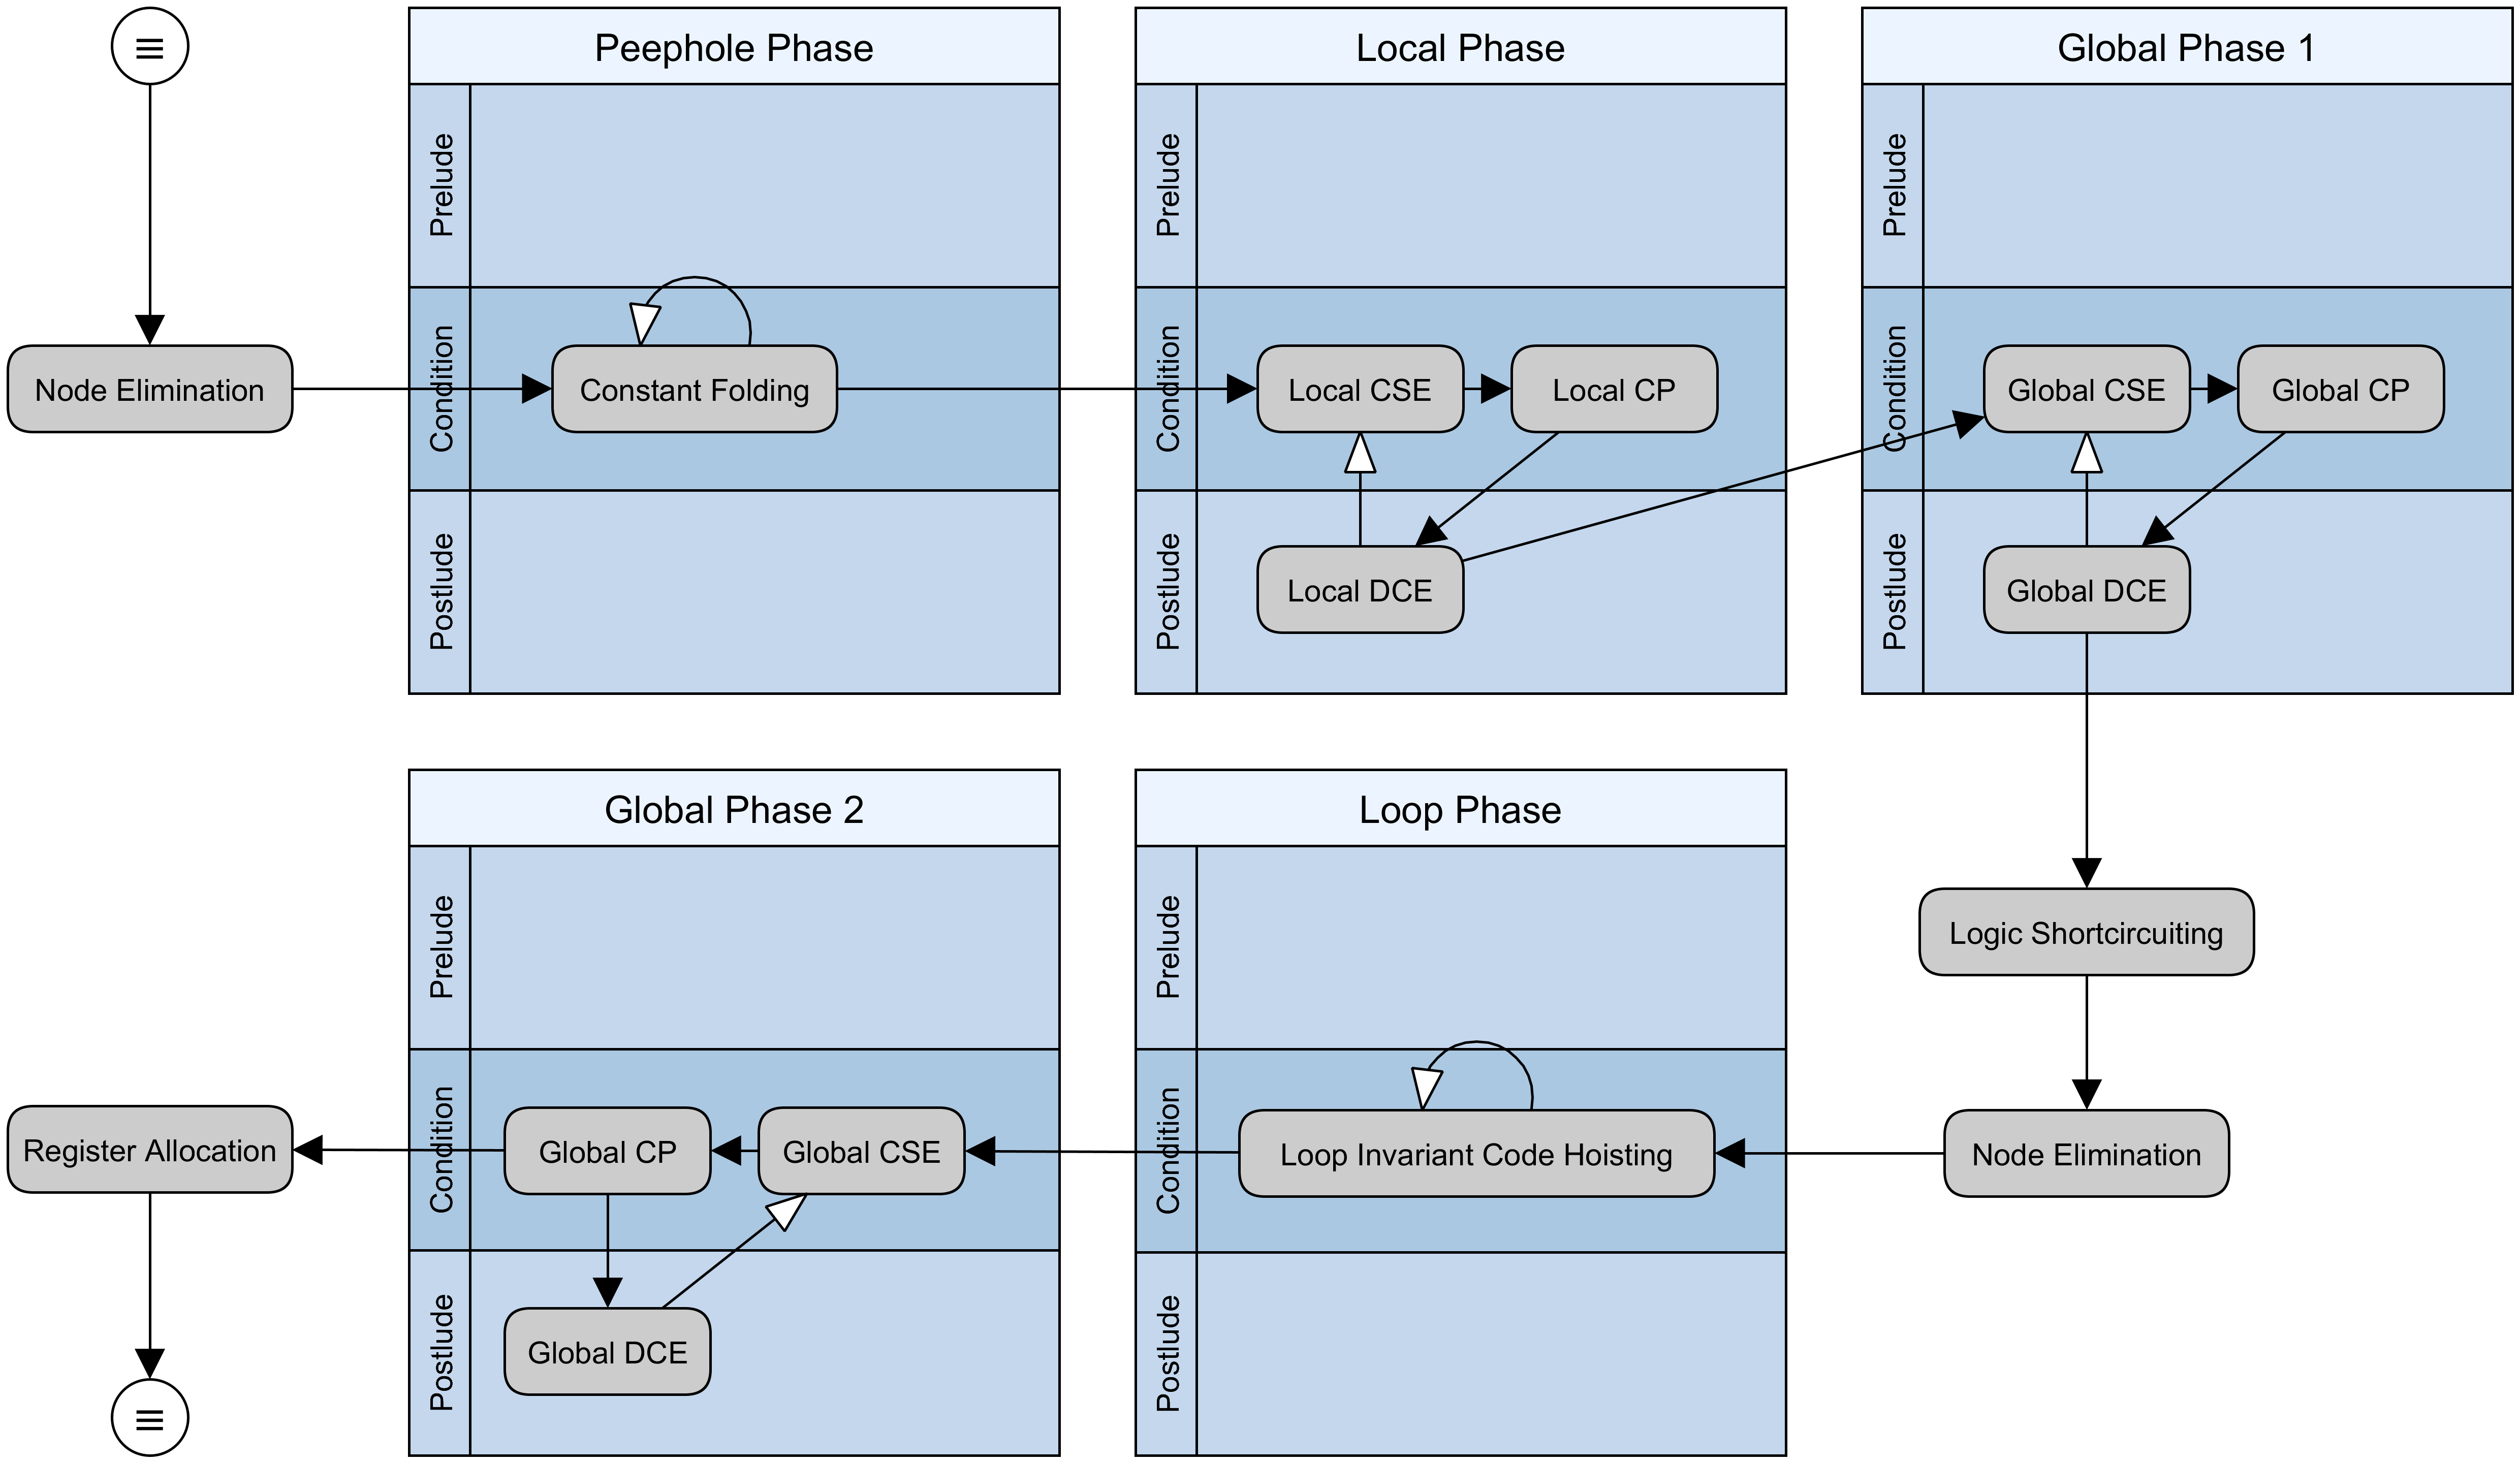
\includegraphics[width=\textwidth]{img/optimization-scheduling}
    \caption{Complete optimization workflow of the Scalars Decaf Compiler}
    \label{fig:optimization-scheduling}
\end{figure}

Figure \ref{fig:optimization-scheduling} demonstrates the complete optimization workflow of the compiler program.

\section{Register Allocation}

\subsection{Introduction}

Register allocation is implemented to move load/store operations from the memory to registers. Since register accesses often offer a significant speedup over memory accesses, this optimization helps reduce time-per-instruction and thus improve performance.

\subsection{Implementation Details}

Register allocation is implemented in line with L22. The implementation files can be found as |src/optimization/reg_alloc/*|. The procedure for finding def-use chains is implemented in |DefUseChain.scala| and |DUChainConstruct.scala|. For each method, the program identifies each valid def-use pair and add computes the convex set of each pair. Afterwards, def-use webs are constructed from the def-use pairs. Implementation for constructing def-use webs is in |DefUseWeb.scala| and |DUWebConstruct.scala|. A union-find algorithm is employed to consolidate def-use chains by referring to their convex sets. After def-use webs are constructed, we employ the Lavrov-Chaitin heuristic to greedily color the def-use webs (c.f. |WebGraphColoring.scala|). Webs that are uncolorable are spilled to memory, while others are each assigned a unique register. In determining which webs to spill, we calculate the spill cost by considering all loops within a convex set of a web, as well as any nesting of such loops. A multiplicative factor of $10$ is applied for each level. The assigned registers are then employed in translating the CFG to assembly code.

\subsection{Demonstration}

For the following sample program, we provide the assembly code generated with and without register allocation. Note that all other optimizations mentioned above are applied.

\begin{lstlisting}[language=C]
    import printf;

    int read_int() {
        return 1;
    }

    void main() {
        int a, b, c, d;
        a = read_int();
        b = read_int();
        if (a > b) {
            c = a + read_int();
        }
        else {
            d = a + read_int();
        }
        printf("%d\n", a);
    }
\end{lstlisting}

\begin{itemize}
    \item Without register allocation:
    \begin{lstlisting}
        .bss
        .text
        .globl read_int
        read_int:
            enter $0, $0
        _3_r0_c0_Block_Init:
            movq $1, %rax
            leave
            ret
        _2_r3_c5_Method_ed:
            jmp noReturn
        .globl main
        main:
            enter $-24, $0
        _6_r0_c0_Block_Init:
        _9_r9_c9_call_call:
            xor %rax, %rax
            call read_int
            addq $0, %rsp
        _9_r9_c9_call_block:
            movq %rax, -8(%rbp)
        _12_r10_c9_call_call:
            xor %rax, %rax
            call read_int
            addq $0, %rsp
        _12_r10_c9_call_block:
            movq %rax, -16(%rbp)
            movq -8(%rbp), %rdx
            movq -16(%rbp), %rsi
            xor %rax, %rax
            cmpq %rsi, %rdx
            setg %al
            movzbl %al, %eax
            movq %rax, -24(%rbp)
        _13_r11_c5_If_cond:
            movq -24(%rbp), %rax
            test %rax, %rax
            je _25_r0_c0_Block_Init
        _18_r0_c0_Block_Init:
        _23_r12_c17_call_call:
            xor %rax, %rax
            call read_int
            addq $0, %rsp
        _23_r12_c17_call_block:
            jmp _32_r17_c5_call_call
        _25_r0_c0_Block_Init:
        _30_r15_c17_call_call:
            xor %rax, %rax
            call read_int
            addq $0, %rsp
        _30_r15_c17_call_block:
            jmp _32_r17_c5_call_call
        _32_r17_c5_call_call:
            movq $str_r17_c12, %rdi
            movq -8(%rbp), %rsi
            xor %rax, %rax
            call printf
            addq $0, %rsp
        _32_r17_c5_call_block:
        _5_r7_c6_Method_ed:
            movq $0, %rax
            leave
            ret
        .globl noReturn
        noReturn:
            movq $-2, %rdi
            call exit
        .globl outOfBound
        outOfBound:
            movq $-1, %rdi
            call exit
        .section .rodata
            str_r17_c12:
                .string "%d\n"        
    \end{lstlisting}
    \item With register allocation:
    \begin{lstlisting}
        .bss
        .text
        .globl read_int
        read_int:
            enter $0, $0
        _3_r0_c0_Block_Init:
            movq $1, %rax
            leave
            ret
        _2_r3_c5_Method_ed:
            jmp noReturn
        .globl main
        main:
            enter $-24, $0
        _6_r0_c0_Block_Init:
        _9_r9_c9_call_call:
            xor %rax, %rax
            call read_int
            addq $0, %rsp
        _9_r9_c9_call_block:
            movq %rax, %r13
        _12_r10_c9_call_call:
             push %r13
            xor %rax, %rax
            call read_int
            addq $0, %rsp
             pop %r13
        _12_r10_c9_call_block:
            movq %rax, %r12
            movq %r13, %rdx
            movq %r12, %rsi
            xor %rax, %rax
            cmpq %rsi, %rdx
            setg %al
            movzbl %al, %eax
            movq %rax, %rbx
        _13_r11_c5_If_cond:
            movq %rbx, %rax
            test %rax, %rax
            je _25_r0_c0_Block_Init
        _18_r0_c0_Block_Init:
        _23_r12_c17_call_call:
             push %r13
            xor %rax, %rax
            call read_int
            addq $0, %rsp
             pop %r13
        _23_r12_c17_call_block:
            jmp _32_r17_c5_call_call
        _25_r0_c0_Block_Init:
        _30_r15_c17_call_call:
             push %r13
            xor %rax, %rax
            call read_int
            addq $0, %rsp
             pop %r13
        _30_r15_c17_call_block:
            jmp _32_r17_c5_call_call
        _32_r17_c5_call_call:
             push %r13
            movq $str_r17_c12, %rdi
            movq %r13, %rsi
            xor %rax, %rax
            call printf
            addq $0, %rsp
             pop %r13
        _32_r17_c5_call_block:
        _5_r7_c6_Method_ed:
            movq $0, %rax
            leave
            ret
        .globl noReturn
        noReturn:
            movq $-2, %rdi
            call exit
        .globl outOfBound
        outOfBound:
            movq $-1, %rdi
            call exit
        .section .rodata
            str_r17_c12:
                .string "%d\n"        
    \end{lstlisting}
\end{itemize}

Observe that the loading/storing of variables now occur on registers, rather than on the stack.

\section{Difficulties}
\begin{enumerate}
    \item Implementing array support for local and global optimizations.
\end{enumerate}

\section{Contribution}

\subsection{Allen Mi}
\begin{enumerate}
    \item Implemented local CSE, local CP, global CSE and optimization scheduling.
    \item Implemented array support for local and global optimizations.
    \item Cooperatively completed register allocation.
    \item Debugging.
    \item Completed documentation.
\end{enumerate}

\subsection{Hanxiang Ren}
\begin{enumerate}
    \item Implemented local DCE, global CP, global DCE, constant folding and loop invariant code hoisting.
    \item Cooperatively completed register allocation.
    \item Debugging.
\end{enumerate}

\end{document}
